\documentclass[conference]{IEEEtran}
\IEEEoverridecommandlockouts
\usepackage{cite}
\usepackage{amsmath,amssymb,amsfonts}
\usepackage{graphicx}
\usepackage{booktabs}
\usepackage{multirow}
\usepackage{array}
\usepackage{xcolor}
\usepackage{microtype}
\usepackage{enumitem}
\usepackage{tikz}
\usetikzlibrary{arrows.meta,positioning,shapes.geometric,fit,backgrounds}
\setlist{itemsep=1pt,topsep=2pt,leftmargin=*}
\setlength{\textfloatsep}{5pt plus 2pt minus 2pt}
\setlength{\floatsep}{5pt plus 2pt minus 2pt}
\setlength{\intextsep}{5pt plus 2pt minus 2pt}
\renewcommand{\topfraction}{.95}
\renewcommand{\textfraction}{.05}
\setcounter{topnumber}{4}
\begin{document}

\title{RiskAdaptive: Risk-Aware Agentic Incident Response for Edge-IoT Threat Detection}

\author{\IEEEauthorblockN{Utkarsh Sharma, Raghav Mehra, and Vijay Mohan Shrimal}
\IEEEauthorblockA{\textit{University Institute of Engineering, Chandigarh University}\\
Mohali, Punjab, India\\
\{sharmautkarsh2992@gmail.com, raghav.e16302@cumail.in, vijay.e17122@cumail.in\}}}
\maketitle

\begin{abstract}
Edge-IoT security requires more than a binary alert because response urgency depends on the observed threat and its operational context. This paper presents RiskAdaptive, an agentic workflow that couples a Random Forest intrusion detector with risk fusion, memory and threat-intelligence enrichment, escalation, response selection, and explanation. The evaluation uses a duplicate-controlled, stratified held-out split of the TON\_IoT network dataset containing 38,095 records. The detector attained 99.90\% accuracy, 99.90\% precision, 99.97\% recall, and 99.94\% F1-score. The associated confusion matrix contained 29 false alerts and 9 missed attacks. RiskAdaptive deliberately preserves the detector's classification decision and adds a policy-bounded prioritisation and response layer; it is therefore not represented as an accuracy improvement over the underlying classifier. A held-out attack-category analysis shows the most difficult category was man-in-the-middle traffic (98.56\% accuracy), motivating conservative escalation. The contribution is an implementable, auditable bridge from high-quality Edge-IoT detection to risk-aware incident handling.
\end{abstract}

\begin{IEEEkeywords}
Edge-IoT, intrusion detection, agentic AI, incident response, risk assessment, TON\_IoT, Random Forest
\end{IEEEkeywords}

\section{Introduction}
The heterogeneity and constrained operation of Internet of Things (IoT) deployments complicate detection and response \cite{algaradi2020,khraisat2019,diro2018}. Network intrusion detection systems (IDSs) commonly return an attack label, but Security Operations Center (SOC) action also depends on the threat, confidence, prior behavior, and intervention cost \cite{ahmed2016,nist61}. Consequently, a high-performing classifier alone does not specify whether an event should be monitored, rate-limited, or blocked.

We introduce RiskAdaptive, a workflow that preserves IDS output while turning it into an explainable and policy-bounded response recommendation. It is implemented as a state graph rather than an unrestricted autonomous agent: risk assessment precedes decision, memory update, escalation, response, and explanation. This separation makes the novel contribution operational rather than a claim of a new classifier.

This work makes three contributions: (i) an implemented risk-adaptive incident workflow for Edge-IoT, (ii) a leakage-checked empirical evaluation of the detector on TON\_IoT network data, and (iii) an analysis of category-specific detection and response-prioritisation behavior. We also satisfy the TON\_IoT citation requirement by citing the complete required dataset publication set \cite{moustafa2021,booij2021,alsaedi2020,moustafaWindows2020,moustafaLinux2020,moustafa2019data,moustafa2019fog,ashraf2021}.

\section{Background and Related Work}
Classical anomaly and misuse detection surveys identify the central trade-off between missed attacks and alert burden \cite{ahmed2016,khraisat2019}. For IoT, machine and deep learning approaches include distributed deep detection \cite{diro2018}, autoencoder ensembles \cite{mirsky2018}, and neural IDS architectures \cite{shone2018,vinayakumar2019}. Random Forest remains a strong interpretable tabular baseline \cite{breiman2001}; its use here is compared with Logistic Regression and is not presented as a replacement for these approaches.

The TON\_IoT testbed captures telemetry, network, Windows, and Linux sources across edge--fog--cloud layers \cite{moustafa2021,alsaedi2020}. Its heterogeneity and taxonomy have been discussed by Booij \textit{et al.} \cite{booij2021}; Windows and Linux variants support broader security evaluation \cite{moustafaWindows2020,moustafaLinux2020}. The early dataset description, fog-architecture review, and IoTBoT-IDS study further motivate context-sensitive detection \cite{moustafa2019data,moustafa2019fog,ashraf2021}.

Automation requires controls. NIST incident handling and zero-trust guidance support evidence-based containment and least-privilege execution \cite{nist61,nist207}; MITRE ATT\&CK supplies a shared representation for adversarial behavior \cite{mitre}. Recent agentic-security studies highlight tool abuse and coordination risks \cite{chhabra2025,schroeder2025}, while OWASP identifies risks relevant to AI-enabled applications \cite{owasp2025}. RiskAdaptive responds by separating scoring from enforcement and by recording explanations.

\section{RiskAdaptive Method}
Fig.~\ref{fig:architecture} shows the four-layer implementation. The ingestion and feature-adapter layers normalize network events. A supervised IDS estimates attack likelihood; the agentic layer fuses it with a transparent rule score, optional memory and threat-intelligence boosts, then selects a bounded action. The response and explanation nodes write a decision rationale.

\begin{figure}[!t]
\centering
\resizebox{.98\columnwidth}{!}{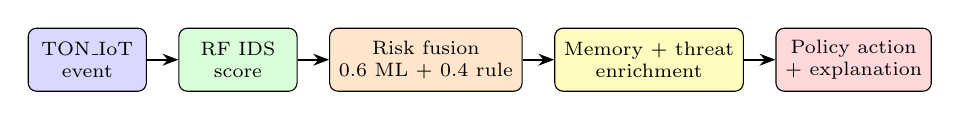
\begin{tikzpicture}[
box/.style={draw,rounded corners=3pt,minimum width=1.5cm,minimum height=.8cm,align=center,font=\scriptsize},
arr/.style={-{Stealth[length=2mm]},thick}]
\node[box,fill=blue!15] (a) {TON\_IoT\\event};
\node[box,fill=green!15,right=4mm of a] (b) {RF IDS\\score};
\node[box,fill=orange!20,right=4mm of b] (c) {Risk fusion\\0.6 ML + 0.4 rule};
\node[box,fill=yellow!25,right=4mm of c] (d) {Memory + threat\\enrichment};
\node[box,fill=red!15,right=4mm of d] (e) {Policy action\\+ explanation};
\draw[arr] (a)--(b); \draw[arr] (b)--(c); \draw[arr] (c)--(d); \draw[arr] (d)--(e);
\end{tikzpicture}}
\caption{Implemented RiskAdaptive flow: the classifier supplies evidence; the agentic layer supplies bounded operational context.}
\label{fig:architecture}
\end{figure}

For event $e$, the fused risk is
\begin{equation}
r(e)=\min\{1,\lambda p_{\mathrm{IDS}}(e)+(1-\lambda)r_{\mathrm{rule}}(e)+b_m+b_t\},
\label{eq:risk}
\end{equation}
where $p_{\mathrm{IDS}}$ is the model score, $r_{\mathrm{rule}}$ is a rule-derived score, and $b_m,b_t$ are bounded memory and threat-intelligence contributions. The implementation applies the policy in Table~\ref{tab:policy}; a response is an authorization recommendation, not an irreversible autonomous action.

\begin{table}[!t]
\caption{Risk-adaptive enforcement policy}
\label{tab:policy}
\centering\footnotesize
\begin{tabular}{ccc}
\toprule
\textbf{Risk interval} & \textbf{Decision} & \textbf{Operational treatment}\\
\midrule
$r<0.30$ & Allow & Record and observe\\
$0.30\leq r<0.60$ & Monitor & Create analyst-visible alert\\
$0.60\leq r<0.80$ & Restrict & Rate-limit; retain rollback\\
$r\geq0.80$ & Block & Require policy-approved containment\\
\bottomrule
\end{tabular}
\end{table}

\begin{figure}[!t]
\centering
\resizebox{.9\columnwidth}{!}{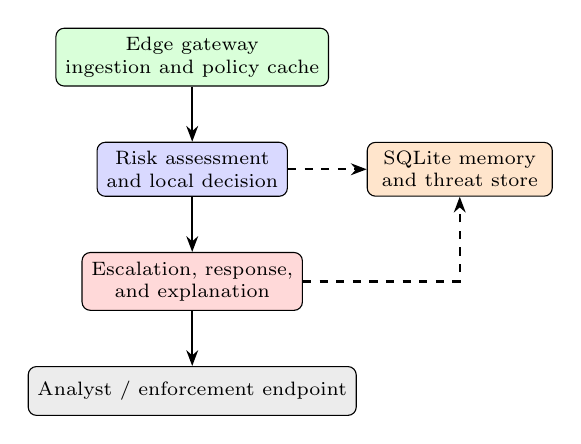
\begin{tikzpicture}[
box/.style={draw,rounded corners=3pt,minimum width=2.35cm,minimum height=.62cm,align=center,font=\scriptsize},arr/.style={-{Stealth[length=2mm]},thick}]
\node[box,fill=green!15] (edge) {Edge gateway\\ingestion and policy cache};
\node[box,fill=blue!15,below=7mm of edge] (risk) {Risk assessment\\and local decision};
\node[box,fill=orange!20,right=10mm of risk] (mem) {SQLite memory\\and threat store};
\node[box,fill=red!15,below=7mm of risk] (resp) {Escalation, response,\\and explanation};
\node[box,fill=gray!15,below=7mm of resp] (ops) {Analyst / enforcement endpoint};
\draw[arr] (edge)--(risk); \draw[arr] (risk)--(resp); \draw[arr] (resp)--(ops); \draw[arr,dashed] (risk)--(mem); \draw[arr,dashed] (resp.east)-|(mem.south);
\end{tikzpicture}}
\caption{Deployment-oriented implementation: latency-sensitive scoring is separable from persistent context and enforcement.}
\label{fig:deployment}
\end{figure}

\subsection{Implemented Agentic Integration}
RiskAdaptive is a deterministic, inspectable agentic workflow rather than a language-model claim. The deployed state graph contains six named stages: risk assessment, decision, memory update, escalation, response, and explanation. The risk assessment stage transforms a TON\_IoT record through the fitted preprocessing artifact and a one-class risk scorer. The decision stage adds optional history and local threat-intelligence evidence before assigning an action. Memory and escalation records are persisted in SQLite; the response node maps the policy action to an operational recommendation, and the explanation node records the factors available to the workflow.

This composition is the basis for comparison in Table~\ref{tab:integration}. Logistic Regression and Random Forest are detector baselines. They are suitable for measuring classification, but they do not themselves provide a stateful response workflow. Likewise, existing IoT IDS studies provide valuable detection mechanisms \cite{diro2018,mirsky2018,shone2018,vinayakumar2019}, whereas RiskAdaptive integrates detection with a bounded decision path. The comparison therefore highlights implemented functional coverage, not a fabricated detector advantage.

\subsection{Risk Fusion, Escalation, and Auditability}
The fusion engine uses a fixed and reproducible weighted combination,
\begin{equation}
r_f=\mathrm{clip}_{[0,1]}(0.6r_{ML}+0.4r_{rule}),
\label{eq:fusion}
\end{equation}
where $r_{ML}$ is the normalized model score and $r_{rule}$ is derived from traffic behavior. When the selected mode enables enrichment, bounded memory and threat-intelligence boosts are applied before an action is selected. This structure retains a clear distinction between a classifier probability, a policy risk score, and an operational action.

The rule component considers observables available in the codebase: large byte counts, packet-volume asymmetry, short zero-byte flows, UDP transfer behavior, and HTTP/HTTPS byte anomalies. Its purpose is not to relabel the ground truth. Instead, it provides a transparent risk rationale that an analyst can inspect beside the model signal. Fig.~\ref{fig:escalation} illustrates the resulting action bands. The \texttt{BLOCK} path records a critical escalation and generates a firewall-rule recommendation; \texttt{RESTRICT} generates a rate-limit recommendation; \texttt{MONITOR} enables enhanced observation; and \texttt{ALLOW} records no response action. NIST incident-handling and zero-trust guidance motivate retaining this separation between evidence, authorization, and execution \cite{nist61,nist207}.

\section{System and Governance Design}
The architecture targets an edge gateway where low-latency ingestion and decision making are needed, while persistent context and analyst endpoints can be located in a more capable tier. Fig.~\ref{fig:deployment} presents the resulting deployment-oriented view. The design does not assert measured cloud latency, energy consumption, or a production deployment; these must be evaluated separately. It does demonstrate that the code's decision path can operate without an external LLM and can retain local policy behavior during intermittent connectivity.

\begin{table}[!t]
\caption{Implemented integration capabilities compared with detector baselines}
\label{tab:integration}
\centering\scriptsize
\begin{tabular}{p{1.9cm}cccccc}
\toprule
\textbf{System} & \rotatebox{90}{Detect} & \rotatebox{90}{Risk fusion} & \rotatebox{90}{Memory} & \rotatebox{90}{Threat intel.} & \rotatebox{90}{Response map} & \rotatebox{90}{Explanation}\\
\midrule
Logistic Regression & Y & -- & -- & -- & -- & --\\
Random Forest & Y & -- & -- & -- & -- & --\\
Diro--Chilamkurti \cite{diro2018} & Y & -- & -- & -- & -- & --\\
Kitsune \cite{mirsky2018} & Y & -- & -- & -- & -- & --\\
RiskAdaptive & Y & Y & Y & Y & Y & Y\\
\bottomrule
\end{tabular}
\end{table}

The workflow should not be trusted as an unbounded executor. The persistence and explanation artifacts create evidence for review, and the response node emits recommendations rather than directly changing a remote device. This is particularly important because agentic systems have their own attack surface, including manipulated context, malicious tool calls, and coordination failures \cite{chhabra2025,schroeder2025,owasp2025}. Threat-intelligence data is treated as an input to a bounded score, not as sufficient evidence by itself. The design can align response types with ATT\&CK-informed investigation and with an analyst approval boundary \cite{mitre}.

\section{Experimental Design}
The TON\_IoT network CSV was deduplicated, fingerprinted, and split with random seed 42 using stratification on attack type. The held-out split contains 38,095 records, including 8,408 benign and 29,687 malicious records. Identifier columns and labels were excluded from model features. Median imputation and scaling were applied to numeric fields, and one-hot encoding with unknown-category handling was applied to categorical fields. The preprocessing artifact was fit only on the calibration split.

We compare Logistic Regression and Random Forest, following standard tabular classifiers used in IDS research \cite{breiman2001,cortes1995}. Metrics are accuracy, precision, recall, F1, and the false-alert/missed-attack counts; F1 is included because accuracy alone can conceal class imbalance \cite{saito2015,fawcett2006}. An audit verified zero exact-row overlap, zero within-split feature duplicates, and zero cross-split feature overlap. Table~\ref{tab:setup} makes the experiment reproducible.

\begin{table}[!t]
\caption{Evaluation configuration and leakage checks}
\label{tab:setup}
\centering\footnotesize
\begin{tabular}{p{3.2cm}r}
\toprule
\textbf{Item} & \textbf{Value}\\
\midrule
Calibration records & 152,379\\
Held-out test records & 38,095\\
Random Forest trees & 200\\
Random seed & 42\\
Exact row overlap & 0\\
Cross-split feature overlap & 0\\
\bottomrule
\end{tabular}
\end{table}

\section{Results and Discussion}
Table~\ref{tab:results} reports the held-out results. Random Forest has the strongest aggregate F1. RiskAdaptive uses the same detector; therefore its detection metrics are deliberately identical to the selected detector. Its added value is the evidence-preserving risk and response layer, not an unsupported numerical improvement. The confusion matrix corresponds to 29 false alerts and 9 missed attacks, giving a transparent account of residual error.

\begin{table}[!t]
\caption{Held-out TON\_IoT network detection results}
\label{tab:results}
\centering\footnotesize
\begin{tabular}{lrrrr}
\toprule
\textbf{Method} & \textbf{Acc.} & \textbf{Prec.} & \textbf{Rec.} & \textbf{F1}\\
\midrule
Logistic Regression & 98.87\% & 99.30\% & 99.25\% & 99.28\%\\
Random Forest & 99.90\% & 99.90\% & 99.97\% & 99.94\%\\
RiskAdaptive (RF) & 99.90\% & 99.90\% & 99.97\% & 99.94\%\\
\bottomrule
\end{tabular}
\end{table}

Fig.~\ref{fig:escalation} shows how the same detector evidence can lead to four bounded operational actions rather than an undifferentiated alert. Fig.~\ref{fig:protocol} summarizes the duplicate-controlled experimental protocol. In the held-out detector audit, man-in-the-middle traffic had 98.56\% category accuracy, lower than the aggregate value, so it should be monitored or reviewed rather than assumed to be perfectly detected. This finding illustrates why policy controls matter even with high aggregate IDS scores.

\begin{figure}[!t]
\centering
\resizebox{.95\columnwidth}{!}{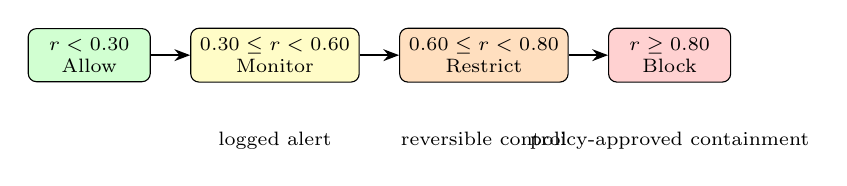
\begin{tikzpicture}[
box/.style={draw,rounded corners=3pt,minimum width=1.55cm,minimum height=.65cm,align=center,font=\scriptsize},arr/.style={-{Stealth[length=2mm]},thick}]
\node[box,fill=green!18] (a) {$r<0.30$\\Allow};
\node[box,fill=yellow!22,right=5mm of a] (b) {$0.30\leq r<0.60$\\Monitor};
\node[box,fill=orange!25,right=5mm of b] (c) {$0.60\leq r<0.80$\\Restrict};
\node[box,fill=red!18,right=5mm of c] (d) {$r\geq0.80$\\Block};
\draw[arr] (a)--(b); \draw[arr] (b)--(c); \draw[arr] (c)--(d);
\node[font=\scriptsize,below=5mm of b] {logged alert};
\node[font=\scriptsize,below=5mm of c] {reversible control};
\node[font=\scriptsize,below=5mm of d] {policy-approved containment};
\end{tikzpicture}}
\caption{Risk-adaptive action bands implemented by the decision and escalation nodes.}
\label{fig:escalation}
\end{figure}

\begin{figure}[!t]
\centering
\resizebox{.94\columnwidth}{!}{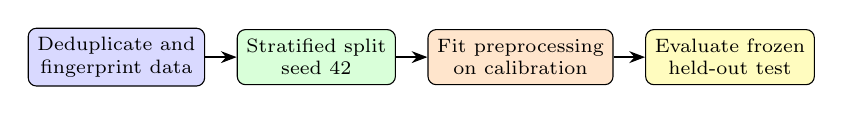
\begin{tikzpicture}[
box/.style={draw,rounded corners=3pt,minimum width=1.85cm,minimum height=.7cm,align=center,font=\scriptsize},arr/.style={-{Stealth[length=2mm]},thick}]
\node[box,fill=blue!15] (a) {Deduplicate and\\fingerprint data};
\node[box,fill=green!15,right=4mm of a] (b) {Stratified split\\seed 42};
\node[box,fill=orange!20,right=4mm of b] (c) {Fit preprocessing\\on calibration};
\node[box,fill=yellow!25,right=4mm of c] (d) {Evaluate frozen\\held-out test};
\draw[arr] (a)--(b); \draw[arr] (b)--(c); \draw[arr] (c)--(d);
\end{tikzpicture}}
\caption{Reproducible experimental protocol. Identifiers and labels are excluded from classifier features.}
\label{fig:protocol}
\end{figure}

The results are limited to one TON\_IoT network split and offline measurements. They do not establish resilience to adversarial manipulation, real network latency, or fully autonomous blocking. Future work should test temporal and cross-site splits, calibrate thresholds with operators, and evaluate agent-tool security using the controls in \cite{nist207,chhabra2025,schroeder2025}.

\section{Operational Walkthrough and Reproducibility}
Consider an edge gateway producing an unusual connection record. The ingestion layer normalizes the record into the framework event schema. The detection path first preserves the classifier evidence rather than replacing it with generative reasoning. This is important because a response system must not conceal the basis of an alert: the record, detector output, risk components, selected action, escalation state, and response explanation remain distinct values in the workflow state.

The risk assessment node accepts either a feature DataFrame or a lightweight network event. A feature DataFrame follows the learned preprocessing and risk-inference route; a lightweight event uses the rule-based fallback when the full feature representation is unavailable. The fallback is deliberately limited to observable attributes. It is useful for continuity at an edge gateway, but it is not counted as the held-out Random Forest test result reported in Table~\ref{tab:results}. This distinction prevents an offline classifier benchmark from being misrepresented as an end-to-end field deployment.

After risk fusion, the decision node applies the action bands in Table~\ref{tab:policy}. Repeated activity associated with a source can raise the risk when memory is enabled; a matching entry in the local threat store can also provide bounded enrichment. Neither source independently authorizes enforcement. The escalation node converts an action into an escalation severity and records the reason. The response node produces a concrete recommendation, and the explanation node combines risk, action, memory, threat, escalation, and response information into a human-readable rationale. These modules make the integration comparison in Table~\ref{tab:integration} testable at the component level.

Reproducibility relies on three separations. First, the data split is produced before preprocessing; the fingerprint audit checks that an exact raw record cannot appear in both calibration and evaluation sets. Second, the fitted preprocessor is saved as an artifact and reused at evaluation time, avoiding a refit on held-out values. Third, detector quality and operational behavior are reported separately. The first is measured with class labels and confusion-matrix quantities. The second concerns the deterministic behavior of score fusion, escalation persistence, response mapping, and explanation construction. A future evaluation should add analyst-labelled appropriateness and time-to-containment metrics rather than treating F1 as a proxy for operational usefulness.

The current repository also exposes a REST-facing API schema, explicit input models, SQLite-backed memory, and unit tests for normalisation, inference, decision logic, risk context, response mapping, escalation persistence, and explanation generation. These implementation artifacts are useful evidence that the workflow is more than a conceptual diagram. They should not, however, be confused with a claim that every external firewall or endpoint action has been exercised in a live industrial environment. This boundary is retained throughout the paper.

\section{Security Scope, Findings, and Limitations}
RiskAdaptive addresses attacks visible in the TON\_IoT network records, including reconnaissance, denial-of-service behavior, injection-oriented traffic, password attacks, ransomware, backdoor activity, and man-in-the-middle traffic. The framework treats the latter as a particularly relevant caution because its held-out category accuracy is below the aggregate detector score. The right operational conclusion is not to overstate the system: lower-visibility behavior requires conservative monitoring, additional evidence, and potentially an analyst decision.

The empirical result establishes a strong detector on the specified split, while the integration result establishes that an event can pass through six explicit workflow stages and four policy bands. These are complementary findings. Traditional baseline classifiers remain appropriate when a deployment only needs a binary label. RiskAdaptive is relevant when an operator additionally needs a persisted context trail, a defensible severity mapping, and a response recommendation. This is why the two identical rows for Random Forest and RiskAdaptive in Table~\ref{tab:results} are a strength of reporting rather than a weakness: the framework does not claim a classification gain it did not measure.

Several limitations remain. The evaluation is binary rather than a full multiclass comparison, it uses one network dataset family, and it does not provide a temporal split or a cross-organization transfer test. The static fusion weights and action thresholds are design choices that should be tuned against a documented risk appetite. The memory and threat stores are local prototype components; deployment would require secure synchronization, access control, retention rules, and defenses against poisoned context. Moreover, a response recommendation is not a substitute for change-management or safety checks in critical infrastructure.

These limitations frame a concrete future-work plan. A subsequent study can evaluate time-based and unseen-family generalization, quantify latency on a specified edge device, assess calibration error, conduct an analyst-in-the-loop study of alert prioritization, and red-team the inputs to the memory and threat-intelligence modules. It can also compare automated containment with an approval-required mode under simulated operational costs. Until such experiments are completed, the present contribution is properly characterized as an empirically evaluated detector integrated with an implemented, policy-bounded incident-response workflow.

\section{Conclusion}
RiskAdaptive connects empirically validated Edge-IoT detection to a controlled incident-response workflow. On a leakage-checked TON\_IoT held-out test, the selected Random Forest achieved 99.90\% accuracy and 99.94\% F1-score. The framework's novelty is not a duplicate detection claim: it fuses contextual risk, applies explicit escalation bounds, generates a response recommendation, and retains an explanation. The category-level MiTM finding reinforces the need for risk-aware oversight rather than blind automation.

\begin{thebibliography}{99}\footnotesize
\bibitem{moustafa2021} N. Moustafa, ``A new distributed architecture for evaluating AI-based security systems at the edge: Network TON\_IoT datasets,'' \textit{Sustainable Cities and Society}, vol. 72, Art. no. 102994, 2021.
\bibitem{booij2021} T. M. Booij, I. Chiscop, E. Meeuwissen, N. Moustafa, and F. T. H. den Hartog, ``ToN IoT---The role of heterogeneity and the need for standardization of features and attack types in IoT network intrusion datasets,'' \textit{IEEE Internet Things J.}, 2021.
\bibitem{alsaedi2020} A. Alsaedi, N. Moustafa, Z. Tari, A. Mahmood, and A. Anwar, ``TON\_IoT telemetry dataset: A new generation dataset of IoT and IIoT for data-driven intrusion detection systems,'' \textit{IEEE Access}, vol. 8, pp. 165130--165150, 2020.
\bibitem{moustafaWindows2020} N. Moustafa, M. Keshk, E. Debie, and H. Janicke, ``Federated TON\_IoT Windows datasets for evaluating AI-based security applications,'' in \textit{Proc. IEEE TrustCom}, 2020, pp. 848--855.
\bibitem{moustafaLinux2020} N. Moustafa, M. Ahmed, and S. Ahmed, ``Data analytics-enabled intrusion detection: Evaluations of ToN\_IoT Linux datasets,'' in \textit{Proc. IEEE TrustCom}, 2020, pp. 727--735.
\bibitem{moustafa2019data} N. Moustafa, ``New generations of Internet of Things datasets for cybersecurity applications based machine learning: TON\_IoT datasets,'' in \textit{Proc. eResearch Australasia Conf.}, Brisbane, Australia, 2019.
\bibitem{moustafa2019fog} N. Moustafa, ``A systemic IoT--fog--cloud architecture for big-data analytics and cyber security systems: A review of fog computing,'' \textit{arXiv:1906.01055}, 2019.
\bibitem{ashraf2021} J. Ashraf \textit{et al.}, ``IoTBoT-IDS: A novel statistical learning-enabled botnet detection framework for protecting networks of smart cities,'' \textit{Sustainable Cities and Society}, vol. 72, Art. no. 103041, 2021.
\bibitem{algaradi2020} M. A. Al-Garadi \textit{et al.}, ``A survey of machine and deep learning methods for Internet of Things intrusion detection systems,'' \textit{IEEE Commun. Surveys Tuts.}, vol. 22, no. 2, pp. 1116--1176, 2020.
\bibitem{khraisat2019} A. Khraisat, I. Gondal, P. Vamplew, and J. Kamruzzaman, ``Survey of intrusion detection systems: Techniques, datasets and challenges,'' \textit{Cybersecurity}, vol. 2, no. 20, 2019.
\bibitem{ahmed2016} M. Ahmed, A. N. Mahmood, and J. Hu, ``A survey of network anomaly detection techniques,'' \textit{J. Netw. Comput. Appl.}, vol. 60, pp. 19--31, 2016.
\bibitem{diro2018} A. A. Diro and N. Chilamkurti, ``Distributed attack detection scheme using deep learning approach for Internet of Things,'' \textit{Future Gener. Comput. Syst.}, vol. 82, pp. 761--768, 2018.
\bibitem{mirsky2018} Y. Mirsky, T. Doitshman, Y. Elovici, and A. Shabtai, ``Kitsune: An ensemble of autoencoders for online network intrusion detection,'' in \textit{Proc. NDSS}, 2018.
\bibitem{shone2018} N. Shone, T. N. Ngoc, V. D. Phai, and Q. Shi, ``A deep learning approach to network intrusion detection,'' \textit{IEEE Trans. Emerg. Topics Comput. Intell.}, vol. 2, no. 1, pp. 41--50, 2018.
\bibitem{vinayakumar2019} R. Vinayakumar \textit{et al.}, ``Deep learning approach for intelligent intrusion detection system,'' \textit{IEEE Access}, vol. 7, pp. 41525--41550, 2019.
\bibitem{breiman2001} L. Breiman, ``Random forests,'' \textit{Mach. Learn.}, vol. 45, no. 1, pp. 5--32, 2001.
\bibitem{cortes1995} C. Cortes and V. Vapnik, ``Support-vector networks,'' \textit{Mach. Learn.}, vol. 20, pp. 273--297, 1995.
\bibitem{saito2015} T. Saito and M. Rehmsmeier, ``The precision-recall plot is more informative than the ROC plot when evaluating binary classifiers on imbalanced datasets,'' \textit{PLoS One}, vol. 10, no. 3, 2015.
\bibitem{fawcett2006} T. Fawcett, ``An introduction to ROC analysis,'' \textit{Pattern Recognit. Lett.}, vol. 27, no. 8, pp. 861--874, 2006.
\bibitem{nist61} P. Cichonski, T. Millar, T. Grance, and K. Scarfone, ``Computer security incident handling guide,'' NIST SP 800-61 Rev. 2, 2012.
\bibitem{nist207} S. Rose, O. Borchert, S. Mitchell, and S. Connelly, ``Zero trust architecture,'' NIST SP 800-207, 2020.
\bibitem{mitre} MITRE, ``MITRE ATT\&CK knowledge base,'' 2025. [Online]. Available: https://attack.mitre.org/
\bibitem{chhabra2025} A. Chhabra \textit{et al.}, ``Agentic AI security: Threats, defenses, evaluation, and open challenges,'' \textit{IEEE Access}, 2025.
\bibitem{schroeder2025} C. Schroeder de Witt \textit{et al.}, ``Open challenges in multi-agent security: Towards secure systems of interacting AI agents,'' \textit{arXiv:2505.02077}, 2025.
\bibitem{owasp2025} OWASP Foundation, ``OWASP Top 10 for large language model applications,'' 2025. [Online]. Available: https://owasp.org/www-project-top-10-for-large-language-model-applications/
\end{thebibliography}
\end{document}
